\documentclass[
	digital, oneside, nosansbold, nocolorbold, nolot, nolof
]{fithesis4}

\usepackage[resetfonts]{cmap}
\usepackage[T1]{fontenc}
\usepackage[english]{babel}
\usepackage[utf8]{inputenc}

\thesissetup{
    date        = \the\year/\the\month/\the\day,
    university  = mu,
    faculty     = fi,
	department  = {Department of Machine Learning and Data Processing},
    type        = mgr,
    author      = Šimon Varga,
    gender      = m,
    advisor     = {prof. RNDr. Luboš Brim, CSc.},
    title       = {%
		Influence maximization in partially specified Boolean networks},
    keywords    = {Boolean networks, mean-field, attractor, control},
    abstract    = {%
        Mean-field approximation methods are successfully used to analyze
        spreading processes in network models, with great utilization in
        epidemic models. There have been attempts to adopt these methods for
        Systems biology models, among others, for Boolean networks, to find the
        most influential system components. Biology experiments often result in
        some level of uncertainty for modeling. Partially specified Boolean
        networks formalize this uncertainty by introducing logical parameters
        to traditional Boolean networks. In this thesis, we target the problem
        of extending the Individual-based mean-field approximation to work with
        those logical parameters and develop a graphical tool for running the
        method on partially specified Boolean networks.
    },
    thanks      = {%
      These are the acknowledgements for my thesis, which can

      span multiple paragraphs.
    },
    bib         = bib.bib,
    facultyLogo = fithesis-fi,
}

\usepackage{makeidx}      %% The `makeidx` package contains
\makeindex                %% helper commands for index typesetting.
%% These additional packages are used within the document:
\usepackage{mathtools}
\usepackage{amsthm}
\usepackage{amssymb}
\usepackage{amsfonts}
\usepackage{IEEEtrantools}
\usepackage{subcaption}
\usepackage{tikz}
\usetikzlibrary{shapes, positioning}
\usepackage{url}      %% Hyperlinks

\usepackage{algorithm2e}
\RestyleAlgo{ruled}
\SetKwProg{Fn}{function}{:}{end}
\SetKwComment{Comment}{/* }{ */}
\SetKw{Break}{break}
\SetKw{Return}{return}
\LinesNumbered

\usepackage{floatrow} %% Putting captions above tables
\floatsetup[table]{capposition=top}
\usepackage[babel]{csquotes} %% Context-sensitive quotation marks
\graphicspath{ {./images/} }


\theoremstyle{definition}
\newtheorem{definition}{Definition}

\theoremstyle{definition}
\newtheorem{example}{Example}

\newenvironment{ldefinition}
    {\begin{definition}}
	{\par\hspace{\stretch{1}}$\spadesuit$\hspace{\stretch{1}}
     \par\end{definition}}

\newenvironment{lexample}
    {\begin{example}}
    {\par\hspace{\stretch{1}}\rule{0.2\textwidth}{0.01ex}\hspace{\stretch{1}}
     \par\end{example}}


\DeclareMathOperator{\stg}{stg}
\DeclareMathOperator{\bdd}{bdd}
\DeclareMathOperator{\attrf}{attr}
\DeclareMathOperator{\dsetf}{dset}
\DeclareMathOperator{\im}{Im}
\DeclareMathOperator*{\argmin}{arg\,min}

\NewDocumentCommand{\BN}{m}{\mathcal{#1}}
\NewDocumentCommand{\BNRs}{m}{\mathcal{#1}} % BN Regulations
\NewDocumentCommand{\BNUFs}{m}{\mathcal{#1}} % BN Update Functions
\NewDocumentCommand{\state}{m}{\mathtt{#1}} % State (for triplets 101, ...)
\NewDocumentCommand{\attr}{m}{\mathcal{#1}} % Attractor

\NewDocumentCommand{\PBN}{m}{\mathfrak{#1}}
\NewDocumentCommand{\PBNUFs}{m}{\mathfrak{#1}} %PBN Update Functions
\NewDocumentCommand{\paronset}{m}{\mathfrak{#1}} % PARametrizatiON SET
\NewDocumentCommand{\paron}{m}{\mathcal{#1}} % PARametrizatiON
\NewDocumentCommand{\unf}{m}{#1_{\textrm{un}}} % UNinterpreted Function

\NewDocumentCommand{\BNt}{m}{\to_{\BN{#1}}} % BN transition
\NewDocumentCommand{\BNtc}{m}{\rightsquigarrow_{\BN{#1}}} % transitive closure

\NewDocumentCommand{\dset}{m}{\mathfrak{#1}} % driver set
\NewDocumentCommand{\dsetsp}{}{\mathbb{D}} % space of driver sets
\NewDocumentCommand{\dsetfmacro}{m}{\dsetf_{\attr{#1}}}

\NewDocumentCommand{\dom}{m}{\mathcal{D}(#1)} % domain
\NewDocumentCommand{\pset}{m}{\mathrm{P}(#1)} % power set
\NewDocumentCommand{\cnt}{m}{\texttt{\#}(#1)} % count

\NewDocumentCommand{\bddn}{m}{\mathcal{#1}} % bdd notation
\NewDocumentCommand{\bddp}{m}{\bddn{#1}_{\text{p}}} % bdd for parametrizations
\NewDocumentCommand{\bdduf}{m}{\bddn{#1}_{\text{uf}}} % bdd for update functions

\DeclarePairedDelimiter{\set}{\{}{\}}
\DeclarePairedDelimiter{\card}{|}{|}



\begin{document}

\chapter{Introduction}

\paragraph{Systems biology}

A common trait among all humans is a desire to know, to understand. Aristotle
(384--322~BC) described this desire in his work Metaphysics~\cite{aristotle}:

\blockquote[Aristotle]{All men by nature desire to know. An indication of this
    is the delight we take in our senses; for even apart from their usefulness
    they are loved for themselves; and above all others the sense of sight. For
    not only with a view to action, but even when we are not going to do
    anything, we prefer sight to almost everything else. The reason is that
    this, most of all the senses, makes us know and brings to light many
    differences between things.}

A human ambition to see, to explore the world around and inside us has emerged
into many sciences -- one of them being biology, a scientific study of life.
There is a visible trend of \emph{reductionism} interweaving the history of
biology. In the 17th century, René Descartes (1596--1650) stated that complex
systems could be understood by looking into the smaller parts inside the system
and then reassembly them into the whole. Although biology has not yet existed
back then as a scientific discipline of today and the main areas affected by
Descartes' idea of reductionism were mathematics and physics, he also published
his notion of non-human animals being complex automatons designed by a God. He
claimed that such an automaton can be described in a reductionist and
mechanistic way.~\cite{systems_bio_hist, de_homine}

A change in this concept arose in the early part of the 20th century. An
influential work by Norbert Wiener (1894--1964) asked for more system-level
understanding~\cite{cybernetics}.  Many biologists expressed objections against
reductionist attitudes~\cite{woodger_biological, weiss_problem, ludwig_open}. A
new language was used, with dominant terms like complexity, organization,
uniqueness, emergence, unpredictability, and interconnectedness. Reductionistic
and mechanistic biology lacks a view of the vital orchestration of components.
Against reductionism, another paradigm started to be articulated more --
\emph{holism}, coined by Jan Smuts (1870--1950), naturalist, philosopher, and
twice Prime Minister of South Africa~\cite{smuts_holism}.

Although these two theories -- reductionism and holism -- are often put in
contrast to each other, no opposition but reconciliation is needed. It is
important to explore the smaller subsystems, tiny components, and how they
function on their own (reductionism). However, it is not less important to look
at the system from above to explore possible emergent features resulting from
the interplay between components (holism).~\cite{systems_bio_hist}

A nice example is an aggregate motion of a flock of birds.
Reynolds~\cite{reynolds_flock} published a computer simulation where each
agent-bird behaves accordingly to a relatively simple set of rules. A
reductionist scientist could explore these rules and understand the bird's sole
behavior but could not find any evidence among the rules of the amazing
phenomenon because it emerges from the interactions between the components
(birds). A set of simple rules orchestrating the components emerged in the
complex behavior of the whole system -- this is something central to a new
approach in biology rising from holism: \emph{Systems biology}.

To study even a small entity -- a cell -- from the system-wide perspective, one
has to combine interactions of many components on different levels: genome,
transcriptome, proteome, and metabolome space. Processing such a huge amount of
information requires computational methods and software infrastructure,
critical components for systems biology research.~\cite{kitano_overview,
systems_bio_methods}

\paragraph{Boolean networks}

Systems biology models of living systems' dynamics may be categorized as
qualitative or quantitative. An example of a qualitative model is a set of ODE
(ordinary differential equations) precisely describing the kinetics of
processes in the system. Experimental inference of all the kinetic parameters
is usually a complex task. At this place, systems biology benefits from
qualitative models. This work targets one concrete: \emph{Boolean networks}
(BN). BN is a simple model introduced by Stuart Kauffman in 1969 for genetic
regulatory networks (GRN), consisting of simple boolean variables for
components of the GRN (proteins, genes, and metabolites) and discrete relations
between them.  Each variable represents the component being active or not. If
the component is a gene, then the variable represents whether the gene is
transcribed or not. In the case of metabolites or proteins, it may represent
whether the amount of metabolite or protein is sufficient for some reaction.
Boolean functions define the relations between the
variables.~\cite{concepts_bn} Even after such a modeling reduction from the
real-world living system, BNs still may illustrate various processes such as
heart development~\cite{heart_development} and aging of organisms~\cite{aging}.

BNs play an important role in systems biology, but it is often hard to infer
the boolean functions controlling the system. A knowledge that some protein
\(a\) and \(b\) activate another protein \(c\) is insufficient because both
boolean functions \(a \land b\) and \(a \lor b\) are consistent with the
knowledge. This uncertainty may be expressed in a \emph{partially defined
boolean network} (also \emph{parametrized boolean networks}), a more general version of BN.

\paragraph{Attractors and control}

One crucial question about any system is: \enquote{How will the system look
after a long time? Will it settle and not change anymore?} The state the system
will eventually evolve into and never leave is called an \emph{attractor}. Such
a state does not have to be single; an attractor may also consist of multiple
states. In that case, the system switches among the states and visits each
infinitely often, but again, only those states in the attractor, no others.. In
the context of systems biology, an attractor is called a \emph{phenotype} as
well.

Finding a control strategy that drives the system to a desired attractor is
beneficial for many applications, for example, identifying key therapeutic
targets for controlling pathways of regulatory and signaling networks,
providing a basis for designing \emph{in vitro} cell reprogramming experiments,
and many more~\cite{control_psbn}. It is known that this problem is
\(\mathcal{NP}\)-hard in general for boolean networks, but effective
approximations exist ranging from linear to cubic time
complexities~\cite{control_akutsu}. Last year, T.~Parmer et~al. presented an
article~\cite{infl_max_BN} with a novel approximation approach based on a
well-studied problem of \emph{influence maximization} for spreading processes
in social networks.

\paragraph{Our contribution}

The last cited article about influence maximization became a stimulus for this
thesis. T.~Parmer later published
\cite{parmer_dynamical}~and~\cite{parmer_phd}, elaborating more on influence
and control in network-based models. However, to the best of our knowledge, no
attempt to generalize to parametrized boolean networks has been published yet.
Thus, in this work, we aim to adjust their idea to work with PBNs, benchmark on
a suitable set of networks, and design a simple, user-friendly GUI to analyze
models of the user's choice.


\chapter{Preliminaries}

This chapter provides theoretical background related to our work, all the
definitions with examples to facilitate understanding, and the final problem
formulation. For a more in-depth description, we refer a reader to other
articles: for boolean networks~\cite{concepts_bn}, for parametrized
BNs~\cite{kadlecaj_thesis}, and finally for controlling BNs~\cite{infl_max_BN}.
The definitions and notions in our work are adopted from those articles.

\section{Boolean network}

The introduction chapter presented boolean networks in an informal, intuitive
way. Now, we show a solid mathematical definition here.

\begin{ldefinition} \label{def:BN}
A \emph{boolean network} is a 3-tuple $\BN{B} = (V, \BNRs{R}, \BNUFs{F})$,
where:
\begin{description}
\item[$V = \{a, b, c, \ldots \}$] stands for a finite set of
    \emph{boolean variables}, which take on values from $\set{0, 1}$.
\item[$\BNRs{R} \subseteq V^2$] is a set of regulations $(a, b)$. We write
    that the variable $a$ \emph{regulates} the variable $b$, meaning $a$
    appears in the update function for $b$. \emph{Context} of a variable
    $a$ is a set of its regulators
    \[C_{\BN{B}}(a) = \set{b \mid (b, a) \in \BNRs{R}}\]
    We write just $C(a)$ instead of $C_{\BN{B}}(a)$, when it is unambiguous.
\item[$\BNUFs{F}$] is a total mapping from $V$ to a set of
    \emph{update functions}. An update function for variable $v \in V$ is
    denoted as $\BNUFs{F}_v$ and takes a value of every variable in $v$'s
    context as an input and outputs an \emph{update value} for the variable
    $v$.
    \[
        \BNUFs{F}_v \in \set*{F \mid F: \set{0, 1}^{C(v)} \to \set{0, 1}}
    \]
\end{description}
\end{ldefinition}

\begin{lexample} \label{example:BN}
In this example we illustrate the previous definition for a simple 3-variable
boolean network depicted in figure~\ref{fig:bn}.
\begin{figure}[!ht]
\centering
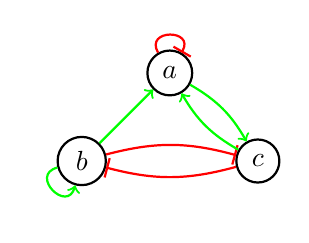
\begin{tikzpicture}[node distance={4.5em}, thick, main/.style = {draw, circle}] 
    \node[main] (a)                        {$a$}; 
    \node[main] (b) [below left of=a]       {$b$};
    \node[main] (c) [below right of=a]        {$c$};

    \draw[red, -|] (a) to [out=120, in=60, looseness=3] (a);
    \draw[relative, green, ->] (a) to [out=15, in=165, looseness=1] (c);

    \draw[green, ->] (b) -- (a);
    \draw[green, ->] (b) to [out=195, in=255, looseness=3] (b);
    \draw[relative, red, -|] (b) to [out=15, in=165, looseness=1] (c);

    \draw[relative, green, ->] (c) to [out=15, in=165, looseness=1] (a);
    \draw[relative, red, -|] (c) to [out=15, in=165, looseness=1] (b);
\end{tikzpicture}
\caption[An example of a BN]{An example of a regulatory graph of a boolean
network. The directed graph is given by the variables and the regulations of
the BN. Here, the edges are moreover colored according to the effect in the
corresponding update function.\label{fig:bn}}
\end{figure}

Clearly, the network contains three boolean variables $\set{a, b, c}$ and
regulations between them:
\[
    \BNRs{R} = \set{(a, a), (a, c), (b, a), (b, b), (b, c), (c, a), (c, b)}
\]

We can define the update functions in multiple ways to be still consistent with
the figure~\ref{fig:bn}. By \enquote{consistent} we mean that for each
regulation $(x, y)$ colored green (red), for every possible valuation of the
other regulators of $y$, changing $x$'s value from 0 to 1 does not change the
value of $\BNUFs{F}_y$ from 1 to 0 (0 to 1, resp.). One of the consistent
definitions is:
\begin{IEEEeqnarray*}{rCl}
    \BNUFs{F}_a(a, b, c) & = & \lnot a \land b \land c\\
    \BNUFs{F}_b(   b, c) & = & b \land \lnot c\\
    \BNUFs{F}_c(a, b   ) & = & a \lor \lnot b
\end{IEEEeqnarray*}

To be more precise in terms of the previous definition, we should write
$\BNUFs{F}_a(\nu) = \lnot \nu(a) \land \nu(b) \land \nu(c)$ instead of
$\BNUFs{F}_a(a, b, c)$ because an update function takes a mapping $\nu: C(a) \to
\{0,1\}$ as a parameter and not the variables $C(a)$ directly. We omit this one
level of indirection for the sake of fluency when reading.

Update functions can also be defined by truth tables:
\[
\begin{array}{ccc|c}
    a & b & c & \BNUFs{F}_a\\
    \hline
    1 & 1 & 1 & 0\\
    1 & 1 & 0 & 0\\
    1 & 0 & 1 & 0\\
    1 & 0 & 0 & 0\\
    0 & 1 & 1 & 1\\
    0 & 1 & 0 & 0\\
    0 & 0 & 1 & 0\\
    0 & 0 & 0 & 0\\
\end{array}
\qquad
\begin{array}{cc|c}
    b & c & \BNUFs{F}_b\\
    \hline
    1 & 1 & 0\\
    1 & 0 & 1\\
    0 & 1 & 0\\
    0 & 0 & 0\\
\end{array}
\qquad
\begin{array}{cc|c}
    a & b & \BNUFs{F}_c\\
    \hline
    1 & 1 & 1\\
    1 & 0 & 1\\
    0 & 1 & 0\\
    0 & 0 & 1\\
\end{array}
\]
\end{lexample}

A BN describes the system structure: main components, and their interactions.
Then, the system evolves and changes its \emph{state} over time according to the
interaction rules -- update functions.

\begin{ldefinition}
A \emph{state} of a boolean network $\BN{B}$ with variables $V$ is a
(total) valuation $\nu : V \to \set{0, 1}$.
\end{ldefinition}

\subsection{Dynamic behavior of boolean networks}

A BN update functions together with \emph{semantics} specifies possible
transitions between states. BN semantics is an \emph{updating policy} for
applying the update functions to a BN's state. There is a wide space for such
policies: the two most common, \emph{synchronous} and \emph{asynchronous}, but
others more sophisticated, synchronous block-sequential, stochastic
asynchronous, and more~\cite{colomoto}. In synchronous semantics, all the
update functions are applied at once. In the asynchronous, only one update
function is used at a time. It was thought that the latter represents
biological systems better, as the components in a living system usually have
concurrent dynamics. Conversely, synchronous updating policy leads to fewer
transitions, and some discussion revealed that it might be more appropriate for
robustness analysis~\cite{concepts_bn}. We made a choice for synchronous
semantics mainly because of the stimulating paper of T.~Parmer~et~al., where
the authors aimed for that policy the most~\cite{infl_max_BN}.

\begin{lexample}
Continuing with the BN from example~\ref{example:BN}, we compare the two most
frequent semantics regarding state $\state{110}$. We write triplet
$\state{110}$ instead of more complex, formal valuation $\set{(a, \state{1}),
(b, \state{1}), (c, \state{0})}$. Asynchronous semantics have two possible
consequent states: $\state{010}$ (after application of $\BNUFs{F}_a$) and
$\state{111}$ ($\BNUFs{F}_c$).  Synchronous semantics have only one:
$\state{011}$.
\end{lexample}

After intuitively describing what semantics is, we provide a definition of
synchronous semantics here:
\begin{ldefinition}
A boolean network $\BN{B} = (V, \BNRs{R}, \BNUFs{F})$ can transition from a
state $\nu_{\text{fr}}$ to a state $\nu_{\text{to}}$ in \emph{synchronous
semantics} if and only if:
\[
    \forall_{v \in V} : \BNUFs{F}_v(\nu_{\text{fr}}\restriction C(v)) =
    \nu_{\text{to}}(v)
\]
Where $\nu\restriction C(v)$ is a restriction of $\nu$ to the domain $C(v)$.

We also define a relation $\BNt{B}$ of feasible transitions, consisting of
all the pairs $(\nu_{\text{fr}}, \nu_{\text{to}})$ such that $\BN{B}$
can change state from $\nu_{\text{fr}}$ to $\nu_{\text{to}}$. We use the notions
$(\nu_{\text{fr}}, \nu_{\text{to}}) \in \BNt{B}$ and
$\nu_{\text{fr}} \BNt{B} \nu_{\text{to}}$ interchangeably.

A transitive closure of $\BNt{B}$ is denoted $\BNt{B}^* = \BNtc{B}$.
\end{ldefinition}

The dynamics of a boolean network can be interpreted as a directed
graph\footnote{\url{https://en.wikipedia.org/wiki/Directed_graph}}, where the
vertices correspond to the states of a BN, and the arcs correspond to the
feasible transitions for a given semantics. The number of vertices is
exponential ($2^{|V|}$) with respect to the number of BN variables because each
variable may (independently) take on two values from~$\set{0, 1}$. There is
always just one outgoing arc from any node for synchronous semantics. From now
on, we consider only synchronous update policy, except we mention the semantics
explicitly.

\begin{ldefinition}
A \emph{state transition graph} (STG) of a BN $\BN{B} = (V, \BNRs{R},
\BNUFs{F})$ is a directed graph $\stg(\BN{B}) = (\mathcal{S}, E)$ with
vertices $\mathcal{S} = \set{0, 1}^V$ and edges $E =\,
\BNt{B} \, \subseteq \mathcal{S}^2$.
\end{ldefinition}

\begin{lexample}
We illustrate the concept of a state transition graph on the BN from
example~\ref{example:BN}. The corresponding STG is depicted in
figure~\ref{fig:STG}. It contains $2^{|V|} = 2^3 = 8$ vertices and the same
number of arcs.
\begin{figure}[!ht]
\centering
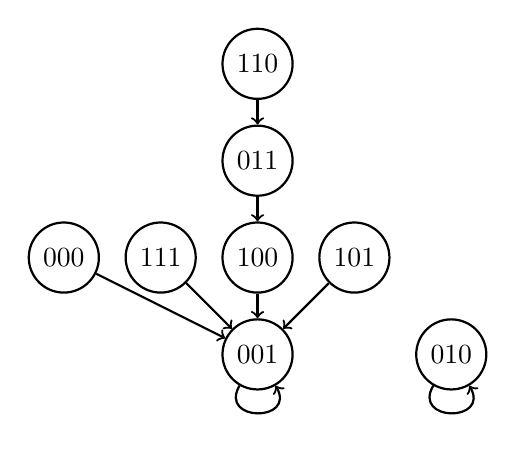
\begin{tikzpicture}[node distance={3.5em}, thick, main/.style = {draw, circle}]
    \node[main] (111) {$\state{111}$};
    \node[main] (000) [left of=111] {$\state{000}$};
    \node[main] (100) [right of=111] {$\state{100}$};
    \node[main] (001) [below of=100] {$\state{001}$};
    \node[main] (011) [above of=100] {$\state{011}$};
    \node[main] (110) [above of=011] {$\state{110}$};
    \node[main] (101) [right of=100] {$\state{101}$};

    \node[main] (010) [right of=001, xshift=3.5em] {$\state{010}$};

    \draw[->] (111) -- (001);
    \draw[->] (011) -- (100);
    \draw[->] (110) -- (011);
    \draw[->] (001) to [out=240, in=300, looseness=3] (001);
    \draw[->] (010) to [out=240, in=300, looseness=3] (010);
    \draw[->] (000) -- (001);
    \draw[->] (101) -- (001);
    \draw[->] (100) -- (001);
\end{tikzpicture}
\caption[An example of a STG]{An example of a state transition graph.}
\label{fig:STG}
\end{figure}
\end{lexample}

In the above example, we can see an interesting feature. The STG contains two
states the system cannot escape from. Component $a$ is absent in both, and
either $b$ or $c$ is active. Moreover, all but one state leads to the final
state $\state{001}$ in the long term. We call them \emph{attractors}, with the
latter having a larger \emph{basin}.

\begin{ldefinition}
An \emph{attractor} of a boolean network $\BN{B}$ is a maximal (finite) set
of states $\attr{A} = \set{\nu_i}_{i=1}^k$ such that:
\[ \forall_{\nu_1, \nu_2 \in \attr{A}} : \nu_1 \BNtc{B} \nu_2 \]

A \emph{basin} of attractor $\attr{A}$ is a (finite) set of all states $\nu$
such that:
\[ \exists_{\nu^{'} \in \attr{A}} : \nu \BNtc{B} \nu^{'} \]
We slightly abuse the notation and write just $\nu \BNtc{B} \attr{A}$.
\end{ldefinition}

\begin{lexample}
For the STG depicted in figure~\ref{fig:STG}, the basin of attractor
$\set{\state{010}}$ is just $\set{\state{010}}$ and the basin of attractor
$\set{\state{001}}$ is a set of all the other vertices.
\end{lexample}


Attractors are categorized based on their size and transitions within. The
simplest case is an attractor containing just one node. It is called a
\emph{fixed-point} attractor. In any other case, the attractor is
\emph{cyclic}. Intuitively, the system cyclically transitions among the states
in a fixed order.

In a synchronous model of the mammalian cell cycle from 2004~\cite{mammalian},
the analysis revealed two attractors: a fixed-point one with a basin of
attraction corresponding to a lack of growth factors, leading to the phase G0
or cell quiescence, and the second one cyclic attractor qualitatively matching
the data and simulation of Novak and Tyson~\cite{novak}. But the synchronous
approach prohibits further refined analysis of the transitions in the cyclic
attractor.

For asynchronous update policy, the categorization is more complex, rising from the fact that the STG contains more edges. Still, the fixed-point attractors coincide with the ones for synchronous policy~\cite{attractors}.

Although T.~Parmer~et~al.~\cite{infl_max_BN} have tried various update
policies, the synchronous one was used to obtain the results presented in their
article that we build on.  It seems to be the most straightforward as well, in
connection to the approximation algorithm they presented. We elaborate more on
this in the next chapter. The article also states that their method, as it is
currently designed, is not usable for cyclic attractors:
\blockquote[T.~Parmer~et~al.~\cite{infl_max_BN}]{Finally, as it is currently
formulated, our method is useful for the study of fixed points only but not
of limit cycles. The method can be generalized to the study of these more
complicated attractors, but only via a non-trivial generalization of our
currently proposed metric of dynamical influence.}

To put it together:
\begin{itemize}
    \item Synchronous semantics leads to simpler STG for analysis.
    \item There is evidence that fixed-point attractors have a more apparent
        analogy to the biological phenotype.
    \item Fixed-point attractors are the same for synchronous and asynchronous
        semantics.
    \item The stimulating article for our thesis works with fixed-points in
        synchronous update policy.
\end{itemize}
Thus we have chosen to focus only on fixed-point attractors and synchronous
semantics.

\subsection{Control of boolean networks}

To ensure that a boolean network reaches a specific, wanted attractor, one has
to interfere with the system if its state transition graph contains multiple
attractors. Such interference is called \emph{perturbation} or \emph{control}.
Two kinds of perturbations exist: state perturbations and update function
perturbations. In the former case, one changes the system's state or restricts
its state space. In the latter case, the STG edges are manipulated by adjusting
the update functions. Usually, it is much less realistic to change a biological
process than to change a system's state, e.g., by adding some
substance~\cite{zanudo}. Therefore we speak only about state perturbations.

State perturbations can be categorized in the following
way~\cite{smijakova_thesis}:
\begin{description}
    \item[One-step] Applied only once, then the system evolves freely due to
        the update policy and functions.
    \item[Temporary] Applied in multiple consequent time steps.
    \item[Permanent] The state space is restricted forever. For example, a
        chosen component cannot be active at all.
\end{description}

\begin{lexample}
When the system in Figure~\ref{fig:STG} settles down in state $\state{010}$
but we would like to have it in the other attractor, $\state{001}$, a
simple one-step control is to change component $a$ to a high state.
Afterward, the system progressively moves from state $\state{110}$ to
$\state{001}$ without any other perturbation because $\state{110}$ lies
in the basin of attraction for $\state{001}$.
\end{lexample}

In our thesis, we are interested in permanent control. It is the most intrusive
and unrealistic one, as it requires forever adding or extracting the
corresponding substance. But, again, the choice has been made regarding the
article~\cite{infl_max_BN} we build on, where the authors work with permanent
perturbations. The control is given by a \emph{driver-set} that drives the
system toward a specific attractor.

\begin{ldefinition}
A \emph{driver-set} $\dset{D}$ for a BN $\BN{B}$ with variables $V$ is a
restriction of (total) valuation $V \to \set{0, 1}$. After application of
$\dset{D}$, the state transition graph $\stg(B)$ is transformed subsequently:
\begin{itemize}
    \item Its vertices are reduced to $V' = \set{\nu \mid \dset{D} \text{ is
        a restriction of } \nu}$. We remind that a function $f$ is a
        restriction of $g$, when:
        \[
        \dom{f} \subseteq \dom{g} \land \forall_{x \in \dom{f}} : f(x) = g(x)
        \]
    \item The edges starting not from $V'$ are removed.
        Each remaining edge $(\nu_{\text{fr}}, \nu_{\text{to}})$ is
        substituted by an edge $(\nu_{\text{fr}}, \nu_{\text{to}}')$,
        such that
        \[
            \nu_{\text{to}}'(v) =
            \begin{cases}
                \dset{D}(v) & \text{if } v \in \dom{\dset{D}},\\
                \nu_{\text{to}}(v) & \text{else}.
            \end{cases}
        \]
        for all $v \in V$. ($\dom{f}$ denotes a domain of a function $f$.)
\end{itemize}

$\dset{D}$ can be interpreted also as a set of $\BN{B}$'s variable
\enquote{fixes}
\[
    \set*{(v, s) \mid v \in V \land s \in \set{0, 1}}.
\]
The space of all driver-sets is denoted by $\dsetsp_{\BN{B}}$.
\end{ldefinition}

\begin{lexample}
Possible driver-sets for the BN defined in Example~\ref{example:BN} are:
$\dset{D_1} = \set{(b, 1)}$, $\dset{D_2} = \set{(b, 1), (c, 0)}$,
or $\dset{D_3} = \set{(b, 0)}$. We depict the related transformations of the STG
in Figure~\ref{fig:STG_transformed} (see the original STG in
Figure~\ref{fig:STG}). $\dset{D_1}$ is not enough to drive the system to
the attractor $\state{010}$ from any state. Adding $(c, 0)$ results in
$\dset{D_2}$ and transforms the $\stg{B}$ to have only one attractor. On the
other side, a driver set $\dset{D_3}$ of size 1 is sufficient to drive the
system toward the other attractor $\state{001}$.
\begin{figure}[!ht]
\centering
\begin{subfigure}{0.3\textwidth}
    \centering
    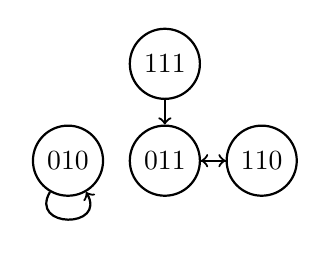
\begin{tikzpicture}[node distance={3.5em}, thick, main/.style = {draw,
                        circle}]
        \node[main] (111) {$\state{111}$};
        \node[main] (011) [below of=111] {$\state{011}$};
        \node[main] (110) [right of=011] {$\state{110}$};

        \node[main] (010) [left of=011] {$\state{010}$};

        \draw[->] (111) -- (011);
        \draw[->] (011) -- (110);
        \draw[->] (110) -- (011);
        \draw[->] (010) to [out=240, in=300, looseness=3] (010);
    \end{tikzpicture}
    \caption{$\set{(b, 1)}$}
\end{subfigure}
\hfill
\begin{subfigure}{0.3\textwidth}
    \centering
    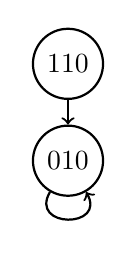
\begin{tikzpicture}[node distance={3.5em}, thick, main/.style = {draw,
                        circle}]
        \node[main] (110) {$\state{110}$};

        \node[main] (010) [below of=110] {$\state{010}$};

        \draw[->] (110) -- (010);
        \draw[->] (010) to [out=240, in=300, looseness=3] (010);
    \end{tikzpicture}
    \caption{$\set{(b, 1), (c, 0)}$}
\end{subfigure}
\hfill
\begin{subfigure}{0.3\textwidth}
    \centering
    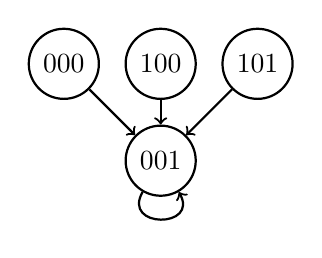
\begin{tikzpicture}[node distance={3.5em}, thick, main/.style = {draw,
                        circle}]
        \node[main] (000) {$\state{000}$};
        \node[main] (100) [right of=000] {$\state{100}$};
        \node[main] (001) [below of=100] {$\state{001}$};
        \node[main] (101) [right of=100] {$\state{101}$};

        \draw[->] (001) to [out=240, in=300, looseness=3] (001);
        \draw[->] (000) -- (001);
        \draw[->] (101) -- (001);
        \draw[->] (100) -- (001);
    \end{tikzpicture}
    \caption{$\set{(b, 0)}$}
\end{subfigure}
\caption{Resulting STGs after a control of given driver-sets.}
\label{fig:STG_transformed}
\end{figure}
\end{lexample}


\section{Mean-field approximations}

The theory of mean-field approximations is mainly adopted from the dissertation
of T.~Parmer~\cite{parmer_phd}.

\emph{Mean-field methods} were originally developed for physics to lower the
number of dimensions of complex models. The idea is to approximate by averaging
(thus \enquote{mean}) over some degrees of freedom in the system. The
component's interactions with many other parts in the model are substituted by
an interaction with this (averaged) \enquote{mean-field}. These methods may
give helpful insight into the system's overall behavior, neglecting local
effects\footnote{A good explanatory (although not practical) example is a
    mean-field approximation of \emph{cellular automata}~\cite{mean_field_ca}.
    The \enquote{mean-field} is just the portion of cells in state~1. Then,
    each cell is supposed to interact with its neighbors, but effectively, only
    a probability of a neighbor being in state~1 is considered (and it is equal
    to the \enquote{mean-field}). The result is a time series of the
    mean-field likelihood.}.

But they are not used only in physics. Approximations using mean-field methods
have been extensively adopted for studying spreading processes on networks,
specifically to address the problem of epidemics~\cite{pastor_epidemic,
yang_epidemic}. The simple SIS
model\footnote{\url{https://en.wikipedia.org/wiki/Compartmental_models_in_epidemiology}}
has two possible types of individuals (also called \emph{compartments}):
Susceptible and Infectious. One can make use of mean-field approximation
provided the population is modeled as infinite and well-mixed.  Then just the
densities of compartments are considered, leading to simple differential
equations. However, the assumption of random interactions among an infinite
number of individuals is only a little applicable to real-world situations.
Therefore, the network models are commonly used, where each individual
interacts with several neighbors. But the network model makes the prediction
computationally harder because a pandemic spreading in a population of size $n$
can be described using a \emph{Markov process} of $n$ random variables $X_i$.
This leads to an exponential number of equations, as $2^n$ possible network
configurations $X = (X_1, X_2, \ldots, X_n)$ exist. Commonly, two methods of
mean-field approximations are used to cope with this exponential explosion:

\begin{description}
    \item[Individual-based] Assumes statistical independence of any two
        neighbors. Informally, when two neighboring individuals $X_1$ and $X_2$
        have a common neighbor $X_3$, he affects both $X_1$ and $X_2$. The
        probability of $X_1(t)$ being infectious is bound to the probability of
        $X_2(t)$ being infectious. The likelihoods depend on each other. But
        this dependence between $X_1$ and $X_2$ is neglected:
        \[
            P(X_1(t) = \text{I} \land X_2(t) = \text{I}) =
            P(X_1(t) = \text{I}) \cdot P(X_2(t) = \text{I}),
        \]
        leading to a simpler formula for a probability of an individual being
        infectious.
    \item[Degree-based] Instead of assuming neighbors are independent, it
        assumes the statistical equality of all the nodes of the same degree.
        Practically, it finds the probability that a node of degree $k$ is in
        a given state at time $t$.
\end{description}

\subsection{Individual-based mean-field approximation for boolean networks}
\label{section:IBMFA}

T.~Parmer~et~al.~\cite{infl_max_BN} presented a novel approach to
individual-based mean-field approximation (IBMFA) applicable to a boolean
network analogic to IBMFA used for pandemic-spreading processes in network
models. The published approximation algorithm aims to estimate the average
dynamics of the system. The brute-force solution would be to consider all
possible initial configurations (states), simulate the dynamics for each one,
and then calculate the average. The time complexity rises fast, as the number
of possible states is exponential to the number of variables.  The proposed
method neglects the dynamic correlations between variables, making the
computation tractable. Here, we shortly describe the method.

\begin{ldefinition}
We describe the \emph{average dynamics} of a BN $\BN{B} = (V, \BNRs{R},
\BNUFs{F})$ by a Markov process $\set*{X}_{t = 0}^T$, where $X(t) =
(X_{v_1}(t), X_{v_2}(t), \ldots, X_{v_n}(t))$ and $\set{v_1, v_2, \ldots,
v_n} = V$. The sample space of a random variable $X_v$ is $\set{0, 1}$. A
probability that the boolean variable $v$ is in the state~1 at time step
$t$ is denoted $\sigma_{v}(t) = P(X_v(t) = 1)$. We call $\sigma(t)$ a
\enquote{\emph{probabilistic state}} or just a \enquote{state} or
\enquote{configuration}, when the distinction from the original notion of a
BN's state is clear from the context.  So, $\sigma(0)$ denotes an initial
configuration. If not specified else, it holds that $\forall_{v \in V} :
\sigma_v(0) = 0.5$.

The dynamics is approximated in the following way:
\begin{equation} \label{eq:ibmfa}
    \sigma_v(t + 1)
    = \sum_{\substack{\nu \in \set{0, 1}^V \\
            \BNUFs{F}_v(\nu\restriction C(v)) = 1}} 
        \prod_{u \in V}
            \left[ \sigma_u(t) \right]^{\nu(u)}
            \cdot \left[ 1 - \sigma_u(t) \right]^{1 - \nu(u)}
\end{equation}
\end{ldefinition}

Now, we assess the time complexity of computing the average dynamics exactly
as opposed to the defined IBMFA:
\begin{description}
    \item[Exact simulation] There are $2^{|V|}$ initial configurations to
        average over. One simulation from the starting configuration
        takes $T$ time-steps.
        Updating the BN's state by one time step during a simulation takes
        in the worst case $|V|^2$ time (updating $V$ variables, each one may
        depend on the previous states of all $V$ variables). Thus the time
        complexity is bounded by $\mathcal{O}(2^{|V|} \cdot T)$.
    \item[IBMFA] According to the work of T.~Parmer~\cite{infl_max_BN},
        one step of the IBMFA simulation runs in time linear with respect to
        $|V|$ (as every variable gets recomputed) and exponential with respect
        to the average degree of nodes in the BN (because there is exponential
        number of valuations for the context of a variable $v$ to sum over
        in Equation~\ref{eq:ibmfa}). Having $T$ iterations of the simulation
        approximation, the complexity is bound by $\mathcal{O}(|V| \cdot 2^k
        \cdot T)$, where $k$ is the average node degree.

        From the view of \emph{parametrized complexity}, we can call an
        algorithm computing IBMFA to be \emph{fixed-parameter
        tractable}\footnote{\url{
        https://en.wikipedia.org/wiki/Parameterized_complexity\#FPT}\\Moreover,
        the problem lies in the FPL (\emph{fixed-parameter linear}) class
        because the network size occurs only as a linear term in the
        derived time complexity.}.  The problem input set may be parametrized
        by the average node degree $k$.  Indeed, in the mentioned article, term
        $2^k$ is neglected, as $k$ is considered to be some low constant.
        Networks in Cell Collective~\cite{cell_collective} repository they have
        been working with are mostly sparse, having $k \approx 2$. This
        practically leads to much better time complexity than the exact
        simulation have: $\mathcal{O}(|V| \cdot T)$.
\end{description}

\begin{lexample}
In the Figure~\ref{fig:simulations}, we illustrate a result of exact and IBMFA
simulations of dynamics of the network from Example~\ref{example:BN}.
The simulations run for 5 iterations. The probabilities in the exact
simulation settled down already in the third iteration. In the IBMFA results,
the probabilities got very close to 0 and 1, so the approximation effectively
ignored the attractor $\state{010}$.
\begin{figure}[!ht]
\centering
\begin{subfigure}{0.85\textwidth}
    \centering
    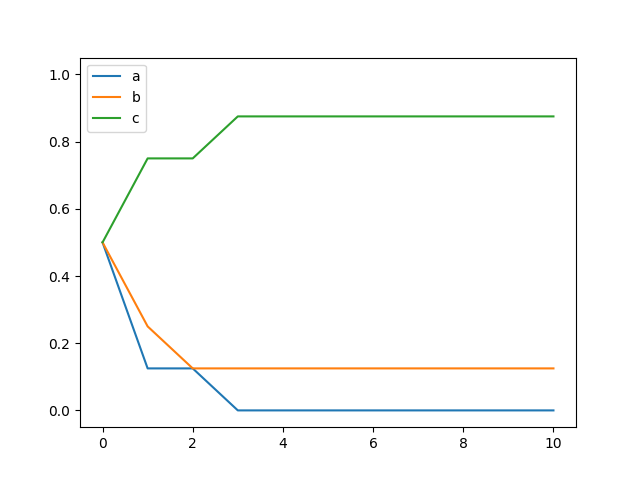
\includegraphics[width=\columnwidth]{example_brute_force.png}
\end{subfigure}
\begin{subfigure}{0.85\textwidth}
    \centering
    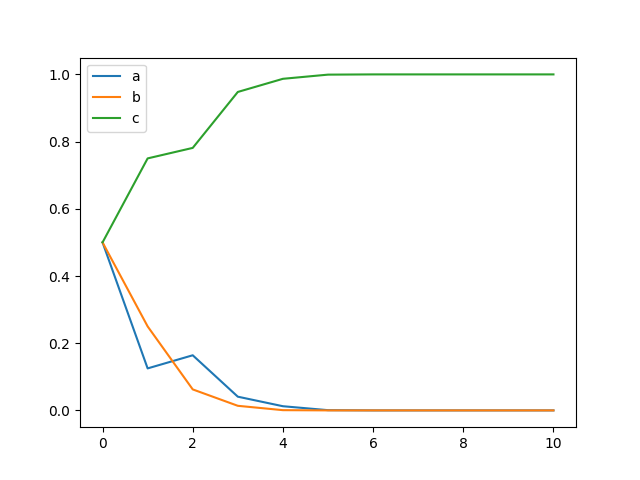
\includegraphics[width=\columnwidth]{example_ibmfa.png}
\end{subfigure}
\caption{Simulation of exact (upper) and IBMFA (bottom) average dynamics
    of BN~\ref{example:BN}}.
\label{fig:simulations}
\end{figure}
\end{lexample}


\subsection{Control of BNs as influence maximization using IBMFA}

Here, we briefly illustrate the utilization of IBMFA~\cite{infl_max_BN} defined
in the previous subsection for finding driver-sets. We adjust the original
equation~\ref{eq:ibmfa} to incorporate driver-sets into the IBMFA simulation.
\begin{ldefinition}
Consider a BN $\BN{B} = (V, \BNRs{R}, \BNUFs{F})$ and a driver-set
$\dset{D} \in \dsetsp_{\BN{B}}$. Then, the IBMFA simulation for BN is defined:
\begin{align*}
    \sigma_v^{\dset{D}}(0) &=
    \begin{cases}
        \dset{D}(v) & \text{if } v \in \dom{\dset{D}},\\
        0.5 & \text{else}.
    \end{cases} \\
    \sigma_v^{\dset{D}}(t + 1) &=
    \begin{cases}
        \dset{D}(v) & \text{if } v \in \dom{\dset{D}},\\
        \sigma_v(t + 1) \text{ as in~\ref{eq:ibmfa}} & \text{else}.
    \end{cases}
\end{align*}
\end{ldefinition}

\begin{figure}[!ht]
\centering
\begin{subfigure}{0.2\textwidth}
    \centering
    \raisebox{7ex}{%
    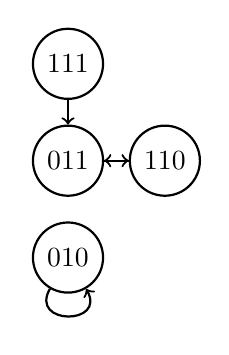
\begin{tikzpicture}[node distance={3.5em}, thick, main/.style = {draw,
                        circle}]
        \node[main] (111) {$\state{111}$};
        \node[main] (011) [below of=111] {$\state{011}$};
        \node[main] (110) [right of=011] {$\state{110}$};

        \node[main] (010) [below of=011] {$\state{010}$};

        \draw[->] (111) -- (011);
        \draw[->] (011) -- (110);
        \draw[->] (110) -- (011);
        \draw[->] (010) to [out=240, in=300, looseness=3] (010);
    \end{tikzpicture}}
\end{subfigure}
\hfill
\begin{subfigure}{0.79\textwidth}
    \centering
    \includegraphics[width=\linewidth]{example_b1.png}
\end{subfigure}
\caption{A state transition graph and IBMFA simulation of boolean network from
    example~\ref{example:BN} for driver-set $\dset{D} = \set{(b, 1)}$.  To
    compare with the dynamics without a driver-set, look at the STG in
    figure~\ref{fig:STG} and simulations in figure~\ref{fig:simulations}. With
    $\dset{D}$, there are still two attractors, but the difference in the size
    of their basins is lesser, so the approximation records both and does not
    settle down to values 0 or 1 as in the situation without $\dset{D}$. The
    probability plot shows that most attractor states have a value of 0 for $a$
    and $c$ and that in the case when it is not so, $a$ and $c$ take on
    opposite values (this is apparent from the alternating local peaks in the
    graph). The corresponding STG supports the same evidence.}
\label{fig:dset_ibmfa}
\end{figure}

A change in IBMFA simulation after setting the driver-set to
$\dset{D} = \set{(b, 1)}$ is depicted in Figure~\ref{fig:dset_ibmfa}.
The result is qualitatively different from the result shown in
Figure~\ref{fig:simulations}, where the probabilities settled down to 0 or 1
after five iterations of IBMFA. To characterize the settledness (or
\emph{uncertainty}) numerically, T.~Parmer~et~al. used entropy.
\begin{ldefinition}
The \emph{uncertainty} of a network configuration in time $t$
is defined as its normalized entropy:
\begin{align*}
    H(X(t)) & = \frac{1}{|V|} \sum_{v \in V} \sum_{s \in \set{0, 1}}
        - P(X(t) = s) \log_2(P(X(t) = s)) \\
        & = \frac{1}{|V|} \sum_{v \in V} \sum_{s \in \set{0, 1}}
            - \sigma_v(t) \log_2\left(\sigma_v(t)\right)
\end{align*}
We write $H(X(t))$ and $H(\sigma(t))$ interchangeably. Note that it is just an
approximation of true entropy, as the dependence between variables is
neglected. The values $H(\sigma(t))$ range from 0 to 1, with a maximum for the
highest uncertainty, e.i. $\forall_{v \in V} : \sigma_v(t) = 0.5$, and a minimum
for any stable configuration $\forall_{v \in V} : \sigma_v(t) \in \set{0, 1}$.
\end{ldefinition}

After fixing a driver-set, the opposite of uncertainty, $1 - H$, is a measure
of the influence of $\dset{D}$ on BN's average dynamics. The lower the
uncertainty, the higher the driver-set's impact on the dynamics. T.~Parmer
proposes a simple greedy search algorithm for finding a minimal driver-set so
that the entropy settles to zero after sufficient iterations of IBMFA. The
authors have experimentally determined the value $T = 10$. We use the same
value in our work.

The pseudocode is shown in Algorithm~\ref{algo:greedy}; a less formal
description follows here. The set of fixes $F$ consistent with the driver set
is prepared at the start. Then, in a loop, one fix is chosen in a greedy
fashion for each iteration to minimize the entropy of the final configuration
in IBMFA. After reaching zero entropy, the driver-set is done. Then, the next
procedure follows -- reducing the driver-set -- to eliminate unnecessary fixes
because the greedy search may build too big a driver-set.

\begin{algorithm}[!ht]
\caption{Greedy search for a driver-set}\label{algo:greedy}
\SetAlgoLined
\KwIn{The attractor $\nu \in \set{0, 1}^V$ to find driver-set for}
\KwOut{Driver-set $\dset{D}$}
$F \gets \nu$\;
$\dset{D} \gets \emptyset$\;
\While{$F \neq \emptyset$}{
    $f \gets \argmin_{f \in F} H(\sigma^{\dset{D} \cup \set{f}}(T))$\;
    $F \gets F \setminus \set{f}$\;
    $\dset{D} \gets \dset{D} \cup \set{f}$\;
    \If{$H(\sigma^{\dset{D}}(T)) = 0$}{
        \Break
    }
}
\While{$\dset{D} \neq \emptyset$}{
    $f \gets \argmin_{f \in \dset{D}}
        H(\sigma^{\dset{D} \setminus \set{f}}(T))$\;
    \If{$H(\sigma^{\dset{D} \setminus \set{f}}(T)) > 0$}{
        \Break
    }
    $\dset{D} \gets \dset{D} \setminus \set{ f }$\;
}
\end{algorithm}

In addition to finding a driver-set for a specific attractor, the original
article mentions an unconstrained version of the algorithm, where all possible
fixes are considered. Thus the resulting driver-set leads to an attractor that
is reached most easily. The only differences in the pseudocode are:
\begin{itemize}
    \item In the preparation of fixes $F$ on line 1.
        \[
            F \gets V \times \set{0, 1}
        \]
    \item In removing a chosen fix $f$ from $F$ on line 5. As $F$ contains
        $(v, 0)$ and $(v, 1)$, both have to be removed, so the other one
        cannot be chosen in a later iteration.
        \[
            F \gets F \setminus \set{(v, 0), (v, 1)}
                \text{ where } (v, \cdot) = f
        \]
\end{itemize}
The authors state the time complexity is cubic with respect to the number of
network nodes $|V|$. It follows from the fact that the size of driver-set can,
in general, grow as fast as $|V|$, so $\mathcal{O}(|V|)$ iterations of the main
loop are run, in each, a minimum over $\mathcal{O}(|V|)$ variables is being
found, and for each variable, the IBMFA simulation gets computed, which takes
time linear to $|V|$.


\section{Parametrized boolean networks}

Estimating the BN's update functions from wet laboratory experiments is often
challenging. It is feasible to generalize the BN concept to work with limited
knowledge about the living system. For example, an inference of an inhibiting
effect of two molecules on the occurrence of another component is insufficient.
The boolean network formalism still requires choosing whether both molecules
together have this effect ($\land$) or if any of them is enough ($\lor$).
However, it would be nice to use at least the knowledge about inhibiting that
we have. A generalization of a BN model to a \emph{parametrized boolean
network}\footnote{The two terms \enquote{partially defined boolean network} and
\enquote{parametrized boolean network} coincide. In the text, we use the later
one, which is shorter.} allows it.

\begin{ldefinition}
A \emph{parametrized boolean network} (PBN) is a 5-tuple
$\PBN{B} = (V, \BNRs{R}, F, \paronset{P}, \PBNUFs{F})$, where:
\begin{description}
    \item $V$ is a set of \emph{boolean variables}.
    \item $\BNRs{R}$ is a set of \emph{regulations} as in ordinary BNs.
    \item $F$ is a set of \emph{parameters}. A parameter is an uninterpreted
        boolean function. To differentiate the notion from interpreted
        functions, we denote a parameter by a label \enquote{un}: $\unf{f}^{n}$
        for $n$-ary uninterpreted function. Thus a parameter consists only
        of a name and assigned arity.
    \item $\paronset{P}$ is a set of valid \emph{parametrizations} -- mappings
        \[
            F \to \set*{ f \mid f : \set{0,1}^n \to \set{0,1},
                n \in \set{0, 1, 2, \ldots} }
        \]
        An image of a parameter $\unf{f}^{n} \in F$ in some parametrization
        $\paron{P} \in \paronset{P}$ is an \emph{interpretation} of
        $\unf{f}^{n}$:
        \[
            \paron{P}(\unf{f}^{n}): \set{0, 1}^n \to \set{0, 1}
        \]
    \item $\PBNUFs{F}$ is a set of \emph{parametrized update functions} $\set*{
        \PBNUFs{F}_v \mid v \in V }$. A boolean expression $\PBNUFs{F}_v$, as
        opposed to (non-parametrized) update function $\BNUFs{F}_v$, may
        contain uninterpreted functions from $F$.
\end{description}
\end{ldefinition}

We introduce a new notation for instantiations of PBNs. For a given
parametrization $\paron{P} \in \paronset{P}$:
\begin{description}
    \item $\PBNUFs{F}_v[\paron{P}]$ denotes an instantiated
        update function arising from interpreting every $\unf{f}$ used in the
        boolean expression $\PBNUFs{F}_v$, as $\paron{P}(\unf{f})$.
        The result is an ordinary update function $\BNUFs{F}_v : \set{0,
        1}^{C(v)} \to \set{0, 1}$.
    \item $\PBNUFs{F}[\paron{P}]$ is equal to $\set{
        \PBNUFs{F}_v\left[\paron{P}\right] \mid v \in V }$.
    \item $\PBN{B}[\paron{P}]$ is an instantiation of a PBN
        $\PBN{B}$ in the parametrization $\paron{P}$. The result is a boolean
        network $\left(V, \BNRs{R}, \PBNUFs{F}\left[\paron{P}\right]\right)$.
\end{description}

\begin{lexample} \label{example:PBN}
This example illustrates the definition of a PBN by transforming the BN
$\BN{B} = (V, \BNRs{R}, \BNUFs{F})$ from Example~\ref{example:BN} into
a parametrized boolean network $\PBN{B} = (V, \BNRs{R}, F, \paronset{P},
\PBNUFs{F})$. We preserve the activating/inhibiting character of regulations
depicted in Figure~\ref{fig:bn} and parametrize the update function for $b$.
We define:
\begin{align*}
    F & = \set{\unf{f}^2} \\
    \paronset{P} & = \set{\paron{P}_1, \paron{P}_2} \\
    \paron{P}_1(\unf{f}^2) & = (x, y) \mapsto x \land \lnot y \\
    \paron{P}_2(\unf{f}^2) & = (x, y) \mapsto x \lor \lnot y \\
    \PBNUFs{F}_x & =
        \begin{cases}
            (a, b, c) \mapsto \unf{f}(b, c) & \text{if } x = b,\\
            \BNUFs{F}_x & \text{else}.
        \end{cases} \\
\end{align*}
Thus there are two BNs $\PBN{B}[\paron{P}_1]$ and $\PBN{B}[\paron{P}_2]$
with different update functions for $b$, $\BNUFs{F}_b = b \land \lnot c$
and $\BNUFs{F}_b = b \lor \lnot c$, respectively. An STG for
$\PBN{B}[\paron{P}_1]$ is depicted in Figure~\ref{fig:STG}
and for $\PBN{B}[\paron{P}_2]$ in Figure~\ref{fig:STG2}.
\begin{figure}[!ht]
\centering
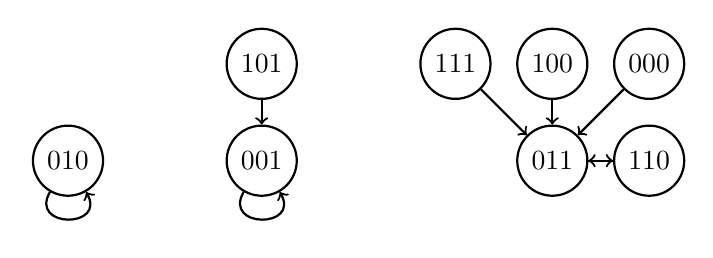
\begin{tikzpicture}[node distance={3.5em}, thick, main/.style = {draw, circle}]
    \node[main] (010) {$\state{010}$};

    \draw[->] (010) to [out=240, in=300, looseness=3] (010);

    \node[main] (001) [right of=010, xshift=3.5em] {$\state{001}$};
    \node[main] (101) [above of=001] {$\state{101}$};

    \draw[->] (001) to [out=240, in=300, looseness=3] (001);
    \draw[->] (101) -- (001);

    \node[main] (011) [right of=001, xshift=7em] {$\state{011}$};
    \node[main] (110) [right of=011] {$\state{110}$};
    \node[main] (100) [above of=011] {$\state{100}$};
    \node[main] (111) [left of=100] {$\state{111}$};
    \node[main] (000) [right of=100] {$\state{000}$};

    \draw[->] (111) -- (011);
    \draw[->] (011) -- (110);
    \draw[->] (110) -- (011);
    \draw[->] (000) -- (011);
    \draw[->] (100) -- (011);
\end{tikzpicture}
\caption{A state transition graph for parametrization $\paron{P}_2$ in
    Example~\ref{example:PBN}.}
\label{fig:STG2}
\end{figure}
\end{lexample}

\section{Problem formulation}
In this thesis, we target the problem of finding driver-sets via IBMFA in
parametrized boolean networks. We aim at the following:
\begin{enumerate}
    \item Given a PBN $\PBN{B}$, find an (approximate) minimal driver-set
        $\dset{D} \in \dsetsp_{\PBN{B}}$ such that $\dset{D}$ drives the
        network $\PBN{B}[\paron{P}]$ to a specific attractor $\nu$ for every
        parametrization $\paron{P}$. We call such $\dset{D}$ a \emph{strong
        driver-set}. Note that different parametrizations may result in
        distinct STG attractors, so we consider only parametrizations resulting
        in a network having $\nu$ among its attractors.
    \item Compute a partition of the parametrization space defined by the
        minimal driver set equivalence. In other words, each partition contains
        all parametrizations $\paron{P}$ in which the network
        $\PBN{B}[\paron{P}]$ has the same minimal driver-set for a given
        attractor.
    \item Implement user-friendly tools for running IBMFA for PBNs and the two
        analyses above.
    \item Benchmark our solution on a suitable set of parametrized boolean
        networks.
\end{enumerate}

\chapter{Computational approach}

We stated our goals and introduced the related concepts in the previous
chapter. Here, we present algorithms and data structures used to accomplish the
goals.

\section{Representing PBNs}

An uninterpreted boolean function of arity $n$ has $2^n$ possible inputs
valuations. The function may output two values for each input, 0 or 1. Thus
$\unf{f}^n$ used in defining a PBN's update function has $2^{2^n}$ possible
instantiations when not restricted by some regulations induced by the
experimental biological data. This \emph{super-exponential} explosion of the
parametrizations makes the explicit representation of a PBN practically
intractable. To deal with this challenging property, we build on the work of
J.~Kadlecaj, who presented a tool for PBN bifurcation analysis in his master's
thesis~\cite{kadlecaj_thesis}. He approached the problem using \emph{Reduced
Ordered Binary Decision Diagram} (ROBDDs, or short: BDDs).

\paragraph{Binary Decision Diagrams}

BDDs are a well-known data structure for working with boolean functions. A BDD
is based on a binary, directed rooted tree, where the decision nodes correspond
to the boolean variables occurring in the represented function. The tree
contains only two terminal nodes connected to boolean values 0 and 1. They tell
the function output for an input containing decision nodes on the path from the
root to a leaf. Each node has two edges, called \emph{low} and \emph{high},
corresponding to a valuation of the node's variable, 0 and 1, respectively.

Interesting properties are the polynomial complexity of applying a binary
logical operation on two BDDs and the space complexity of a BDD. Although, in
the worst case, the tree still takes $\mathcal{O}(2^n)$ space for an $n$-ary
boolean function, the used space is smaller in many cases.

An $n$-ary boolean function $f$ may also be interpreted as a set of $n$-tuples.
The set contains all tuples that are mapped to value 1 by $f$. A set operations
$\cup$, $\cap$, $( )^\complement$ correspond to logical $\lor$, $\land$,
$\lnot$. Thus BDDs are used to represent sets as well.

We use a notation $\bddn{B} = \bdd(f)$ for a BDD representing function $f$.

\paragraph{Representing uninterpreted functions}

For each row in a truth table of $\unf{f}^n$, there is one boolean variable in
a BDD. The constraints are added to BDD according to valid parametrizations of
the PBN.
\begin{lexample}
Continuing with Example~\ref{example:PBN}, we illustrate a BDD for $\unf{f}^2$.
Arity 2 results in four boolean variables for each row in the truth table:
$f_{00}$, $f_{01}$, $f_{10}$, and $f_{11}$. For example, a condition $f_{00} =
0$ restricts to instantiations $f$ of $\unf{f}^2$, where $f(0, 0) = 0$. A BDD
consisting only of a terminal node 1 (or 0) then represents a set of all
possible instantiations (or empty set, respectively). A BDD restricted to
allowed parametrizations is depicted in Figure~\ref{fig:BDD}.

\begin{figure}[!ht]
\centering
\begin{subfigure}{0.45\textwidth}
\centering
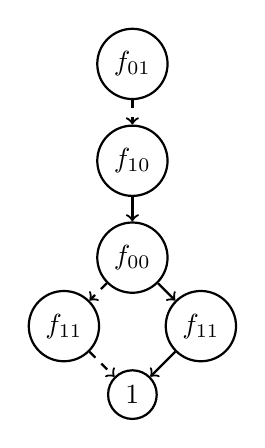
\begin{tikzpicture}[node distance={3.5em}, thick, main/.style = {draw, circle}]
    \node[main] (01) {$f_{01}$};
    \node[main] (10) [below of=01] {$f_{10}$};
    \node[main] (00) [below of=10] {$f_{00}$};
    \node[main] (11a) [below left of=00] {$f_{11}$};
    \node[main] (11b) [below right of=00] {$f_{11}$};
    \node[main] (1) [below right of=11a] {$1$};

    \draw[dashed, ->] (01) -- (10);
    \draw[->] (10) -- (00);
    \draw[dashed, ->] (00) -- (11a);
    \draw[->] (00) -- (11b);
    \draw[dashed, ->] (11a) -- (1);
    \draw[->] (11b) -- (1);
\end{tikzpicture}
\end{subfigure}
\hfill
\begin{subfigure}{0.45\textwidth}
\centering
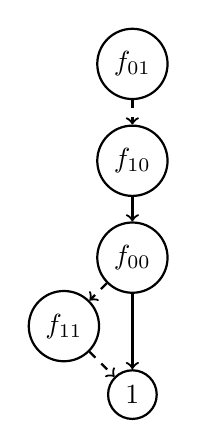
\begin{tikzpicture}[node distance={3.5em}, thick, main/.style = {draw, circle}]
    \node[main] (01) {$f_{01}$};
    \node[main] (10) [below of=01] {$f_{10}$};
    \node[main] (00) [below of=10] {$f_{00}$};
    \node[main] (11) [below left of=00] {$f_{11}$};
    \node[main] (1) [below right of=11] {$1$};

    \draw[dashed, ->] (01) -- (10);
    \draw[->] (10) -- (00);
    \draw[dashed, ->] (00) -- (11);
    \draw[->] (00) -- (1);
    \draw[dashed, ->] (11) -- (1);
\end{tikzpicture}
\end{subfigure}
\caption{A depiction of BDDs with variable ordering $f_{01}$, $f_{10}$,
    $f_{00}$, $f_{11}$. (left) A BDD allowing the two parametrizations
    $\paron{P}_1$ and $\paron{P}_2$, e.i. $x \land \lnot y$ and $x \lor \lnot
    y$.  (right) A BDD after adding a valid parametrization $\paron{P}_3$, that
    maps $\unf{f}^2$ to $(x, y) \mapsto \lnot y$.}
\label{fig:BDD}
\end{figure}
\end{lexample}

\paragraph{Representing update functions}
To store a parametrized update function $\PBNUFs{F}_v$, we need two BDDs: one
for valid parametrizations and one for instantiated update functions. The
former is built as described in the previous section. Boolean variables for
rows of all uninterpreted functions' truth tables used in the boolean
expression $\PBNUFs{F}_v$ are put together into one BDD $\bddp{B}^v$
(\enquote{p} for \emph{p}arametrizations), and the restrictions are applied.
The latter BDD $\bdduf{B}^v$ (\enquote{uf} for \emph{u}pdate \emph{f}unctions)
contains, in addition, variables from the context of $v$. This BDD represents a
function from $\paronset{P} \times \set{0, 1}^{C(v)}$ to $\set{0, 1}$. So it
takes a parametrization and a valuation for the context of $v$, and outputs an
update value for $v$.  The result of $\bdduf{B}^v \land \bdd(g)$ for some
function $g : \dom{\bddp{B}^v} \to \set{0, 1}$ is an update function
$\PBNUFs{F}_v[\paron{P}]$, where $\paron{P} \restriction \set{\unf{f} \mid
\PBNUFs{F}_v \text{ contains } \unf{f}}$ (a restriction takes place here
because $\dom{\paron{P}}$ are all uninterpreted functions used in any
$\PBNUFs{F}_v$) is represented by $g$.

Then, the whole PBN is coded using a BDD $\bddp{B}$ for $\paronset{P}$:
\[
    \bddp{B} = \bigwedge_{v \in V} \bddp{B}^v
\]
and a set of BDDs $\set{\bdduf{B}^v \mid v \in V}$ for $\PBNUFs{F}$. We write
$\dom{\bddp{B}}$ for a domain of $\bddp{B}$, which is a set of all boolean
variables that may occur as internal nodes in $\bddp{B}$.

\section{Finding attractors}

The BDD representation can be utilized straightforwardly to find fixed-point
attractors in synchronous semantics. We introduce an extra variable $v'$ for
each $v$ in $V$. These boolean variables store the \emph{update values} for
BN's variables. We construct a new BDD:
\[
    \bdduf{B} = \bigwedge_{v \in V} \left( \bdduf{B}^v \iff \bdd(v') \right)
\]
We interpret $\bdduf{B}$ as a set of elements (\enquote{parametrization},
\enquote{state}, \enquote{next state}). We filter this set to contain only
elements with valid parametrizations and the same \enquote{state} and
\enquote{next state}, which are the fixed-point attractors:
\[
    \bddp{B} \land \bdduf{B} \land
    \bigwedge_{v \in V} \left( \bdd(v) \iff \bdd(v') \right)
\]
We denote the found attractors by a function $\attrf$ mapping an
attractor $\attr{A}$ to a set of parametrizations, in which the STG contains
$\attr{A}$.

\section{Parametrizations partitioning}

For every attractor $\attr{A}$, we compute a partition of
$\attrf(\attr{A})$, determined by an equivalence relation of
driver-set equality. The result of partitioning is a family of sets:
$\set{\paronset{P}_1, \ldots, \paronset{P}_p}$, such that all BNs
$\set{\PBN{B}[\paron{P}] \mid \paron{P} \in \paronset{P}_i}$ have the same
driver-set for attractor $\attr{A}$. The computation runs in a brute-force
manner iterating over each parametrization $\paron{P} \in
\attrf(\attr{A})$ and finding a driver-set by
Algorithm~\ref{algo:greedy}. We assign the corresponding driver-set to each
$\paronset{P}_i$. Then the result is represented as a mapping $\dsetfmacro{A}:
\dsetsp \to \pset{\attrf(\attr{A})}$. $\pset{X}$ denotes a power set (set of
all subsets) of $X$. By $\cnt{\dsetfmacro{A}}$ we denote total number of mapped
parametrizations $\sum_{\paronset{P} \in \im(\dsetfmacro{A})} |\paronset{P}|$.

This method does not scale well as the number of
parametrizations grows super-exponentially with respect to the number of
regulators $|C(v)|$ and exponentially with respect to the number of BN's
variables $|V|$. Therefore, it is suitable just for an analysis of
small-to-medium models.

To characterize the diversity of found driver-sets $\dsetfmacro{A}$
numerically, we employ normalized (binary) entropy:
\begin{align} \label{formula:entropy}
    H(\dsetfmacro{A})
    &= - \sum_{\paronset{P} \in \im(\dsetfmacro{A})}
        \frac{|\paronset{P}|}{N} \log_2 \frac{|\paronset{P}|}{N} \\
    &= \log_2 N - \frac{1}{N} \sum_{\paronset{P} \in \im(\dsetfmacro{A})}
        |\paronset{P}| \cdot \log_2 |\paronset{P}| \nonumber
\end{align}
$\im{f}$ denotes an image of a function $f$ and $N = \cnt{\dsetfmacro{A}}$.

Entropy has suitable properties. Consider partitioning into $P$, two
parametrizations' groups of size 50. It has an entropy equal to 1. For a more
fine-grained partition, the diversity is of a higher level; we want to express
that numerically. For four groups of size 25, the entropy is 2 --- conversely,
a partition having just one group results in zero entropy. When the number of
groups remains the same as in the original example $P$, but their sizes change
to 25 and 75, then the diversity is lower. For this partition, randomly
choosing one of the driver-sets has a higher probability of taking the
applicable one than for $P$. The entropy changes accordingly, lowers to 0.811.

\subsection{Decision tree induction}

The following task is to explain the partitioning and show differences in the
arisen groups of parametrizations. We approach this problem using decision
trees (DTs)\footnote{\url{https://en.wikipedia.org/wiki/Decision_tree}}. A DT,
similarly to BDD, is based on a directed rooted tree. Its internal nodes serve
as a test for some attributes with outgoing edges for possible test outcomes.
The leaves represent the final class. Decision trees are commonly used as a
data mining method~\cite{data_mining}. Learning decision trees from data is
done step-wise, starting from the root node and developing towards the leaves
recursively. The pseudocode is presented in Algorithm~\ref{algo:dt}. We used
the conventional \emph{information gain} condition for splitting decision
nodes~\cite{decision_trees}. As information gain is just a reduction of
entropy, we minimize the posterior entropy instead of maximizing information
gain. In our setting, a leaf contains a driver-set, and an internal (decision)
node consists of a boolean variable from $\dom{\bddp{B}}$.

\begin{algorithm}[!ht]
\caption{Building a decision tree for parametrizations partition}
\label{algo:dt}

\SetAlgoLined
\SetKwFunction{Split}{split}
\SetKwFunction{CondEntropy}{cond\_H}
\SetKwFunction{MakeDT}{make\_DT}

\KwOut{\MakeDT{$\dsetfmacro{A}, \dom{\bddp{B}}$}}
\BlankLine
\Fn{\MakeDT{$\dsetf, X$}}{
    \KwIn{$\dsetf$ to create a DT for, using decision variables from $X$.}
    \KwOut{A DT $(V, E, R)$ with nodes $V$, edges $E$, and root $R$.
        An edge $e \in E$ is a 3-tuple
        (\enquote{from}, \enquote{to}, \enquote{test outcome}).}
    \BlankLine
    \If{$\dsetf \text{ is empty }$}{
        \Return $(\set{\emptyset}, \emptyset, \emptyset)$\;\label{algo:empty}
    }
    \If{$\dom{\dsetf} \text{ contains just one element } \dset{D}$}{
        \Return $(\set{\dset{D}}, \emptyset, \dset{D})$\;
    }
    $x \gets \argmin_{x \in X}$ \CondEntropy{$\dsetf, x$}\;
    $X \gets X \setminus \set{x}$\;
    $(\dsetf_l, \dsetf_r) \gets$ \Split{$\dsetf, x$}\;
    $(V_l, E_l, R_l) \gets$ \MakeDT{$\dsetf_l, X$}\;
    $(V_r, E_r, R_r) \gets$ \MakeDT{$\dsetf_r, X$}\;
    \Return $(V_l \cup V_r \cup \set{x},
        E_l \cup E_r \cup \set{(x, R_l, 0), (x, R_r, 1)}, x)$\;
}
\BlankLine
\Fn{\Split{$\dsetf, x$}}{
    \KwOut{$\dsetf$ split when $x = 0$ and $x = 1$}
    \BlankLine
    $\dsetf_l \gets \dset{D} \mapsto \dsetf(\dset{D}) \land (x \iff 0)$\;
    $\dsetf_l \gets \dsetf_l \restriction
        \set{\dset{D} \mid \dsetf_l(\dset{D}) \neq \emptyset}$\;
    $\dsetf_r \gets \dset{D} \mapsto \dsetf(\dset{D}) \land (x \iff 1)$\;
    $\dsetf_r \gets \dsetf_r \restriction
        \set{\dset{D} \mid \dsetf_r(\dset{D}) \neq \emptyset}$\;
    \Return $(\dsetf_l, \dsetf_r)$\;
}
\BlankLine
\Fn{\CondEntropy{$\dsetf, x$}}{
    \KwOut{Conditional entropy $H(\dsetf \mid x)$}
    \BlankLine
    $(\dsetf_l, \dsetf_r) \gets $ \Split{$\dsetf, x$}\;
    \Return $\frac{\cnt{\dsetf_l}}{\cnt{\dsetf}} H(\dsetf_l)
        + \frac{\cnt{\dsetf_r}}{\cnt{\dsetf}} H(\dsetf_r)$\;
}
\end{algorithm}

\subsection{Decision tree postprocessing}
Building a decision tree as described in Algorithm~\ref{algo:dt} may result in
empty leaves (line~\ref{algo:empty}). It happens when a variable chosen for a
decision node does not split $\dsetf$, but only restricts its parametrizations
that still end in the same node (and the other one is an empty leaf). As these
empty nodes does not truly mean empty driver-sets, we need to get rid of them.
The process is described in Figure~\ref{fig:dt_post}.

\begin{figure}[!ht]
\centering
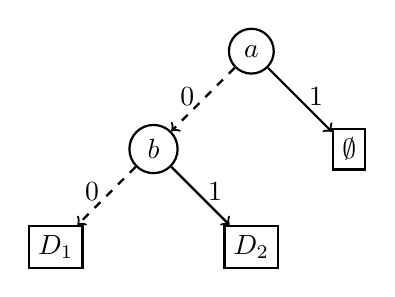
\begin{tikzpicture}[node distance={5em}, thick, node/.style = {draw, circle},
                    leaf/.style = {draw, rectangle}]
    \node[node] (a) {$a$};
    \node[node] (b) [below left of=a] {$b$};
    \node[leaf] (e) [below right of=a] {$\emptyset$};
    \node[leaf] (d1) [below left of=b] {$\dset{D}_1$};
    \node[leaf] (d2) [below right of=b] {$\dset{D}_2$};

    \draw[dashed, ->] (a) -- (b) node [near end, above] {0};
    \draw[->] (a) -- (e) node [near end, above] {1};
    \draw[dashed, ->] (b) -- (d1) node [near end, above] {0};
    \draw[->] (b) -- (d2) node [near end, above] {1};
\end{tikzpicture}
\quad
\quad
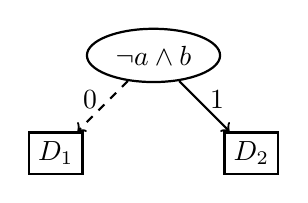
\begin{tikzpicture}[node distance={5em}, thick, node/.style = {draw, ellipse},
                    leaf/.style = {draw, rectangle}]
    \node[node] (ab) {$\lnot a \land b$};
    \node[leaf] (d1) [below left of=ab] {$\dset{D}_1$};
    \node[leaf] (d2) [below right of=ab] {$\dset{D}_2$};

    \draw[dashed, ->] (ab) -- (d1) node [near end, above] {0};
    \draw[->] (ab) -- (d2) node [near end, above] {1};
\end{tikzpicture}
\caption{An example of simple decision tree before (left) and after (right) the
    postprocessing step, that removes the \enquote{empty} driver-set leaves.}
\label{fig:dt_post}
\end{figure}

\section{Strong driver-sets}

To find a driver-set $\dset{D}$ such that for every parametrization $\paron{P}$
in $\attrf{\attr{A}}$, $\dset{D}$ drives $\PBN{B}[\paron{P}]$ toward attractor
$\attr{A}$ (so, \emph{strong driver-set}), we extend the IBMFA method to
average over parametrizations as well. Thus, one \enquote{individual} here is a
randomly initiated configuration and chosen parametrization instead of only a
random configuration for the original IBMFA for BNs.

\begin{ldefinition}
Consider a PBN $\PBN{B} = (V, \BNRs{R}, F, \paronset{P}, \PBNUFs{F})$.
Its average dynamics is approximated in the following way:
\begin{equation}
    \sigma_v(t + 1)
    = \frac{1}{|\paronset{P}|} \sum_{\paron{P} \in \paronset{P}}
        \sum_{\substack{\nu \in \set{0, 1}^V \\
                \PBNUFs{F}_v[\paron{P}](\nu\restriction C(v)) = 1}} 
            \prod_{u \in V}
                \left[ \sigma_u(t) \right]^{\nu(u)}
                \cdot \left[ 1 - \sigma_u(t) \right]^{1 - \nu(u)}
    \label{eq:pbn_ibmfa}
\end{equation}
\end{ldefinition}

We utilize the BDD representation $\bddp{B}$ of $\paronset{P}$ so that we do
not need to iterate over all $\paron{P} \in \paronset{P}$ in the outer-most
sum of formula~\ref{eq:pbn_ibmfa}. For any two $\paron{P}_1, \paron{P}_2 \in
\paronset{P}$, such that $\paron{P}_1(\unf{f}^n) = \paron{P}_2(\unf{f}^n)$ for
all $\unf{f}^n$ used in $\PBNUFs{F}_v$, the instantiated update functions
are equal, $\PBNUFs{F}_v[\paron{P}_1] = \PBNUFs{F}_v[\paron{P}_2]$. Therefore
these two parametrizations contribute to the sum equaly and the outer-most
sum can be changed to:
\[
    \frac{1}{|\paronset{P}'|} \sum_{\paron{P} \in \paronset{P}'}
\]
where $\paronset{P}' = \set{\paron{P}' \mid \paron{P} \in \paronset{P}}$ and
\[
    \paron{P}'(\unf{f}^n) =
        \begin{cases}
            \paron{P}(\unf{f}^n &
                \text{if } \unf{f}^n \text{ is used in } \PBNUFs{F}_v,\\
            (a_1, \ldots, a_n) \mapsto 0 & \text{else}.
        \end{cases}
\]
So, practically, we iterate over satisfying valuations of BDD $\bddp{B}^v$.

\subsection{Time complexity}

The time complexity of computing IBMFA for $T$ time steps is $\mathcal{O}(|V|
\cdot 2^k \cdot T)$, where $k$ is the average node degree (see section~\ref{section:IBMFA}).
Then, calculating the IBMFA explicitly for every parametrization would take
$\mathcal{O}(|V| \cdot 2^k \cdot T \cdot \prod_{v \in V} |\bddp{B}^v|)$
time. Note that $\prod_{v \in V} |\bddp{B}^v|) = |\bddp{B}| =
|\paronset{P}|$. On the contrary, our proposed approximation is bound by:
\[
\mathcal{O}\left(\left[\sum_{v \in V} \card*{\bddp{B}^v}\right]
    \cdot 2^k \cdot T\right)
= \mathcal{O}\left(\left[\max_{v \in V} \card*{\bddp{B}^v}\right]
    \cdot |V| \cdot 2^k \cdot T \right)
\]
When we rewrite the estimate for the explicit computation, we notice
a polynomial improvement:
\[
\mathcal{O}\left(|V| \cdot 2^k \cdot T \cdot
    \prod_{v \in V} \card*{\bddp{B}^v}\right)
= \mathcal{O}\left(\left[\max_{v \in V} \card*{\bddp{B}^v}\right]^{|V|}
    \cdot |V| \cdot 2^k \cdot T\right)
\]


\chapter{Implementation}

This chapter is dedicated to implementation details and a description of
created tools.

The base of our implementation is a Rust library, simply named
\texttt{pbn\_ibmfa}. We have chosen
Rust\footnote{\url{https://www.rust-lang.org/}} as a programming language
mainly because of the useful available libraries \texttt{biodivine-lib-bdd}
used for creating and manipulating BDDs and \texttt{biodivine-lib-param-bn},
which implements a parametrized boolean network representation by BDDs. It
supports us with loading the model files, making all the BDDs, and computing
the restrictions $\paronset{P}$ for them. Further processing is the
responsibility of our library, \texttt{pbn\_ibmfa}. It consists of several
modules:
\begin{description}
\item[\texttt{symbolic\_sync\_graph}] Contains a representation of symbolic
    synchronous STG. Symbolic STG means that just the update functions are
    stored, in the form of BDDs, as described in the previous chapter. This
    module provides the application of constraints given by the input model
    file, basic graph operations, evaluation of update functions, and
    finding attractors.
\item[\texttt{ibmfa\_computations}] Contains entropy computation, IBMFA
    simulation (both versions, for BNs and PBNs), and the entropy minimization
    algorithm.
\item[\texttt{driver\_set}] Implements a driver-set search and parametrization
    partitioning (utilizes the module \texttt{ibmfa\_computations}).
\item[\texttt{decision\_tree}] Contains a definition of the decision tree data
    structure and the Algorithm~\ref{algo:dt} for constructing them from a
    partition of parametrizations.
\item[\texttt{utils}] Simple utility functions, mainly for printing various
    data structures to standard output.
\end{description}

This library is used to implement two user applications for working with PBNs:
one command line and one graphical.

\section{Command line tool \texttt{pbn\_ibmfa}}

The purpose of this command line utility is to run the computations we have presented in our thesis. It takes as input a path to a boolean network file in the \texttt{.aeon} format\footnote{\url{https://biodivine.fi.muni.cz/aeon/}} and prints results of user-selected computations in JSON\footnote{\url{https://www.json.org/json-en.html}} format to standard output. \texttt{pbn\_ibmfa} accepts an argument for producing a JSON with nice spacings and indentations (instead of the default, where the JSON elements are printed in one big chunk of characters). A user may also set the number of iterations used in the IBMFA computing. \texttt{pbn\_ibmfa} takes two subcommands:
\begin{description}
\item[Simulation] The output is a time series of BN's probabilistic
    configurations. Users may choose between IBMFA and exact (brute-force)
    average dynamics. There is a possibility of fixing variables to discover
    the dynamics for diverse driver-sets.
\item[Analysis] Without any other option, it just detects the fixed-point
    attractors. Users may further choose to find a strong driver-set and/or
    driver-sets (and corresponding parametrization partitions) for every
    attractor. Not relating to attractors, \texttt{pbn\_ibmfa} is capable of
    finding the unconstrained strong driver-set (e.i. the one that leads to
    some attractor most quickly). If someone would like to examine driver-sets
    before the postprocessing reduction, he can use the argument
    \verb|--not-reduced|.
\end{description}

\section{Interactive graphical tool}

The implementation is divided into two parts: a client (\emph{front-end}) and a
server (\emph{back-end}). The client is a GUI web application that the user
directly interacts with. The server performs all the intensive computations on
PBNs and communicates with the client. This separation allows the server to run
on a higher-performance computer while the client lives in a browser of an
ordinary desktop computer or laptop.

\subsection{Running the software}

\paragraph{Back-end}

The server is a binary Rust crate using the library \texttt{pbn\_ibmfa}. By
default, it listens on a localhost's port 5678. This setting can be changed via
command line arguments to listen on a different port number and address. After
successful initialization, the server reports it listens on a given address and
port. Then, the server reports an (eventually) successful connection and what
communication with the client is going on (for an ordinary user, that
information is not much important). For reasonably sized models, it is possible
to run the server on a personal computer (we elaborate more on this in the
chapter~\ref{section:results}).

\paragraph{Front-end}

The client consists of one HTML page \verb|index.html| and several JavaScript
scripts included, ready to be opened in a standard web browser. On a startup,
an almost empty webpage gets displayed, with one input for the port number and
a button for initiating the connection. Afterward, the user is shown an error
message or prompted to choose a file containing the input model. In the case of
an invalid file format, the model is rejected, and information is given to the
user about the error. For valid PBN, the numbers of variables and
parametrizations are shown, together with a new button for finding the
attractors. All these interactions are done on a \enquote{Status bar} side
panel. It is depicted, along with other parts of the web application, in
Figure~\ref{fig:web_app}. Now, a description of the individual parts follows.

\begin{figure}[!ht]
\centering
\includegraphics[height=0.7\textwidth, angle=270]{web_application.png}
\caption{A design of the webpage GUI.}
\label{fig:web_app}
\end{figure}

\begin{description}
\item[Status bar] Except for what was already described in the previous
    paragraph, it displays the tool's state, whether it is connected, and if
    some computation is in progress. As the tool is single-threaded, only one
    calculation may run at a time. The bar's bottom part shows a variable name
    corresponding to a variable value in the \enquote{Attractors}'s panel,
    which is hovered over by a mouse pointer.
\item[Attractors] The panel consists of a scrollable table of found fixed-point
    attractors ordered by the corresponding parametrization amount. The amount
    is shown in the column \enquote{colors}\footnote{The name is used in
        connection to
        AEON(\url{https://sybila.fi.muni.cz/tools_html/aeon.html}), where PBN's
    parametrizations are also called colors.} The column \enquote{state} is
    straightforward; it is just a bit vector representing the attractor (e.i.
    each bit corresponds to one PBN's variable). The next two columns are
    initially filled with question marks because it could take a long time to
    compute all those values. Instead, the user chooses which attractor row to
    expand by clicking on it (the row highlighted green in
    Figure~\ref{fig:web_app}). The back-end then finds the strong driver-set
    (shown in the last column -- hyphens are used for variables not contained
    in the strong driver-set) and parametrization partition with assigned
    driver-sets. In the column \enquote{entropy}, a binary entropy for the
    partition is calculated (see Formula~\ref{formula:entropy}).
\item[Decision tree] The rightmost panel depicts a decision tree for the
selected attractor. Each edge is labeled by the corresponding number of
parametrizations. On hovering a node, more context is displayed: for leaves,
names of the variables in the driver-set; for internal nodes, the exact boolean
function contained in the node. Internal nodes are rather labeled by variable
names, whose update function's parametrizations are restricted by the contained
boolean function. We made this decision because labeling by the full boolean
function would draw huge nodes. The user can drag the nodes and reset them to
the original layout by clicking a button. Decision trees are rendered using a
JavaScript visualization library
\texttt{vis.js}\footnote{\url{https://visjs.org/}}.
\end{description}


\chapter{Evaluation} \label{section:results}

This chapter serves for the evaluation of our algorithms. We have used the
command line tool \texttt{pbn\_ibmfa} and benchmarked two processes: finding
strong driver-sets and computing the parametrization partitioning by
driver-sets. The input models can be found on
GitHub\footnote{\url{https://github.com/sybila/biodivine-boolean-models/tree/main}}.
We have run the tool on fully parametrized versions of networks in the GitHub
repository, with the restrictions given by the regulatory graph preserved. The
measurements were conducted on a personal laptop with processor \emph{Intel(R)
Core(TM) i3-3110M CPU @ 2.40GHz} and 8 GB RAM. Below is shown a table of
measured times, PBN model names, and their characteristics:
\begin{itemize}
    \item $|V|$: number of PBN's variables
    \item $|R|$: number of regulations
    \item $|P|$: parameter space size (as displayed in AEON)
\end{itemize}

\begin{tabular}[!ht]{@{}lcccrr@{}}
    \toprule
    Model name & $|V|$ & $|\BNRs{R}|$ & $|\paronset{P}|$ & strong
        $\dset{D}$ & partition \\
    \midrule
    Cortical area development & 5 & 14 & $2^{40}$ & 00:00.67 & 04:29.22 \\
    Asymmetric cell division A & 5 & 15 & $2^{48}$ & 00:01.48 & 17:13.99 \\
    Mir 9 neurogenesis & 6 & 11 & $2^{22}$ & 00:00.04 & 00:00.07 \\
    Trp biosynthesis & 6 & 13 & $2^{37}$ & 00:01.43 & 01:34.40 \\
    P53 MDM2 network & 6 & 15 & $2^{45}$ & 00:02.27 & 37:28.90 \\
    Drosophila gap D & 7 & 12 & $2^{30}$ & 00:00.46 & 00:19.28 \\
    Asymmetric cell division B & 9 & 12 & $2^{24}$ & 00:00.01 & 00:00.04 \\
    Cell cycle transcription & 9 & 19 & $2^{54}$ & 00:01.66 & - \\
    Drosophila wings AP & 10 & 14 & $2^{34}$ & 00:00.64 & 00:23.40 \\
    Root stem cell 2010 & 10 & 16 & $2^{44}$ & >2:30:00 & - \\
    Mammalian cell cycle 2006 & 10 & 34 & $2^{43}$ & >2:30.00 & - \\
    Toll pathway of Drosophila & 11 & 11 & $2^{24}$ & 00:00.03 & 00:00.08 \\
    \bottomrule
\end{tabular}

\medskip

We may conclude that our proposed method is suitable just for
small networks. Doubling the parameter space size seems to have a greater impact
than doubling the variable space size. For networks $|V| > 10$ and
$|\paronset{P}| > 40$ the algorithm is intractable.

\chapter{Conclusion}

This work describes a method of computing individual-based mean-field
approximation on partially specified Boolean networks. We build on the work of
T.~Parmer~et~al.~\cite{infl_max_BN}, who have presented the algorithm for
influence maximization in traditional Boolean networks, taking inspiration from
studying spreading processes in network models -- a pandemic spreading, for
example.

The thesis begins by explaining the related theoretical concepts, Boolean
networks, parametrized Boolean networks, controlling BNs, mean-field methods,
and IBMFA. Then proposes a novel algorithm for computing IBMFA for PBNs and
introduces the notion of a strong driver-set. We designed an algorithm for
explaining the parametrization partitions via decision trees. In the end, we
described tools implemented to analyze PBNs using IBMFA: one command line tool
with more options and one graphical interactive tool that users can run in
their browsers.

\paragraph{Possible improvements}

Analyzing the computation complexity for exemplary PBN models leads to the
conclusion that the approach needs to scale better, mainly for the number of
parametrizations, which grows fast. The tools could benefit from
parallelization up to some point, but rather an innovative enhancement is
necessary.

Except for such a significant change, many minor improvements would improve the
user experience. For example:
\begin{itemize}
\item Reduce the decision tree more. Currently, it is too branched; often, two
    consecutive decision nodes have children leaves containing the same
    driver-set.
\item Show a progress bar in the web application during long server
    computations.
\item Users cannot ask to build the decision tree in the command line tool.
\end{itemize}

\hfil$\spadesuit$\hfil

% TODO is this neccessary?
%\makeatletter\thesis@blocks@clear\makeatother
%\phantomsection %% Print the index and insert it into the
%\addcontentsline{toc}{chapter}{\indexname} %% table of contents.
%\printindex

%\appendix
%\chapter{An appendix}
%Here you can insert the appendices of your thesis.

\end{document}
